\chapter{Rešerše existujích řešení}
\label{sec:nastroje}
Tato kapitola se bude zabývat popisem a srovnáním aktuálně dostupných nástrojů pro tvorbu FMEA. Nejdříve budou krátce představeni tři zástupci aplikací. Následně budou tito tři zástupci srovnání na základě zobecnění základních požadavků na nástroj, který by měl vzniknou v rámci této diplomvé práce. 

Možností pro vypracovná analýzy je více. Nejjednodušší variantou je použití předem definované šablony v libovolném tabulkovém editoru. Tento způsob nabízí velice základní funkce pro vypracování FMEA. Proto je lepší přistuoupit k nějakému profesionálnějšímu řešení, které výrazým způsob usnadňuje a zefektiňuje daný proces. Všechny uvedené nástroje byly vyzkoušeny na základě poskytované demo verze. Při záverečném srovnání bylo bráno v potaz, že některé funkce jsou dostupné až v placených verzích.

\section{Dostupné řešení}
\subsection{FMEA Studio(iQA system)}

\begin{figure}[h]
\centering
	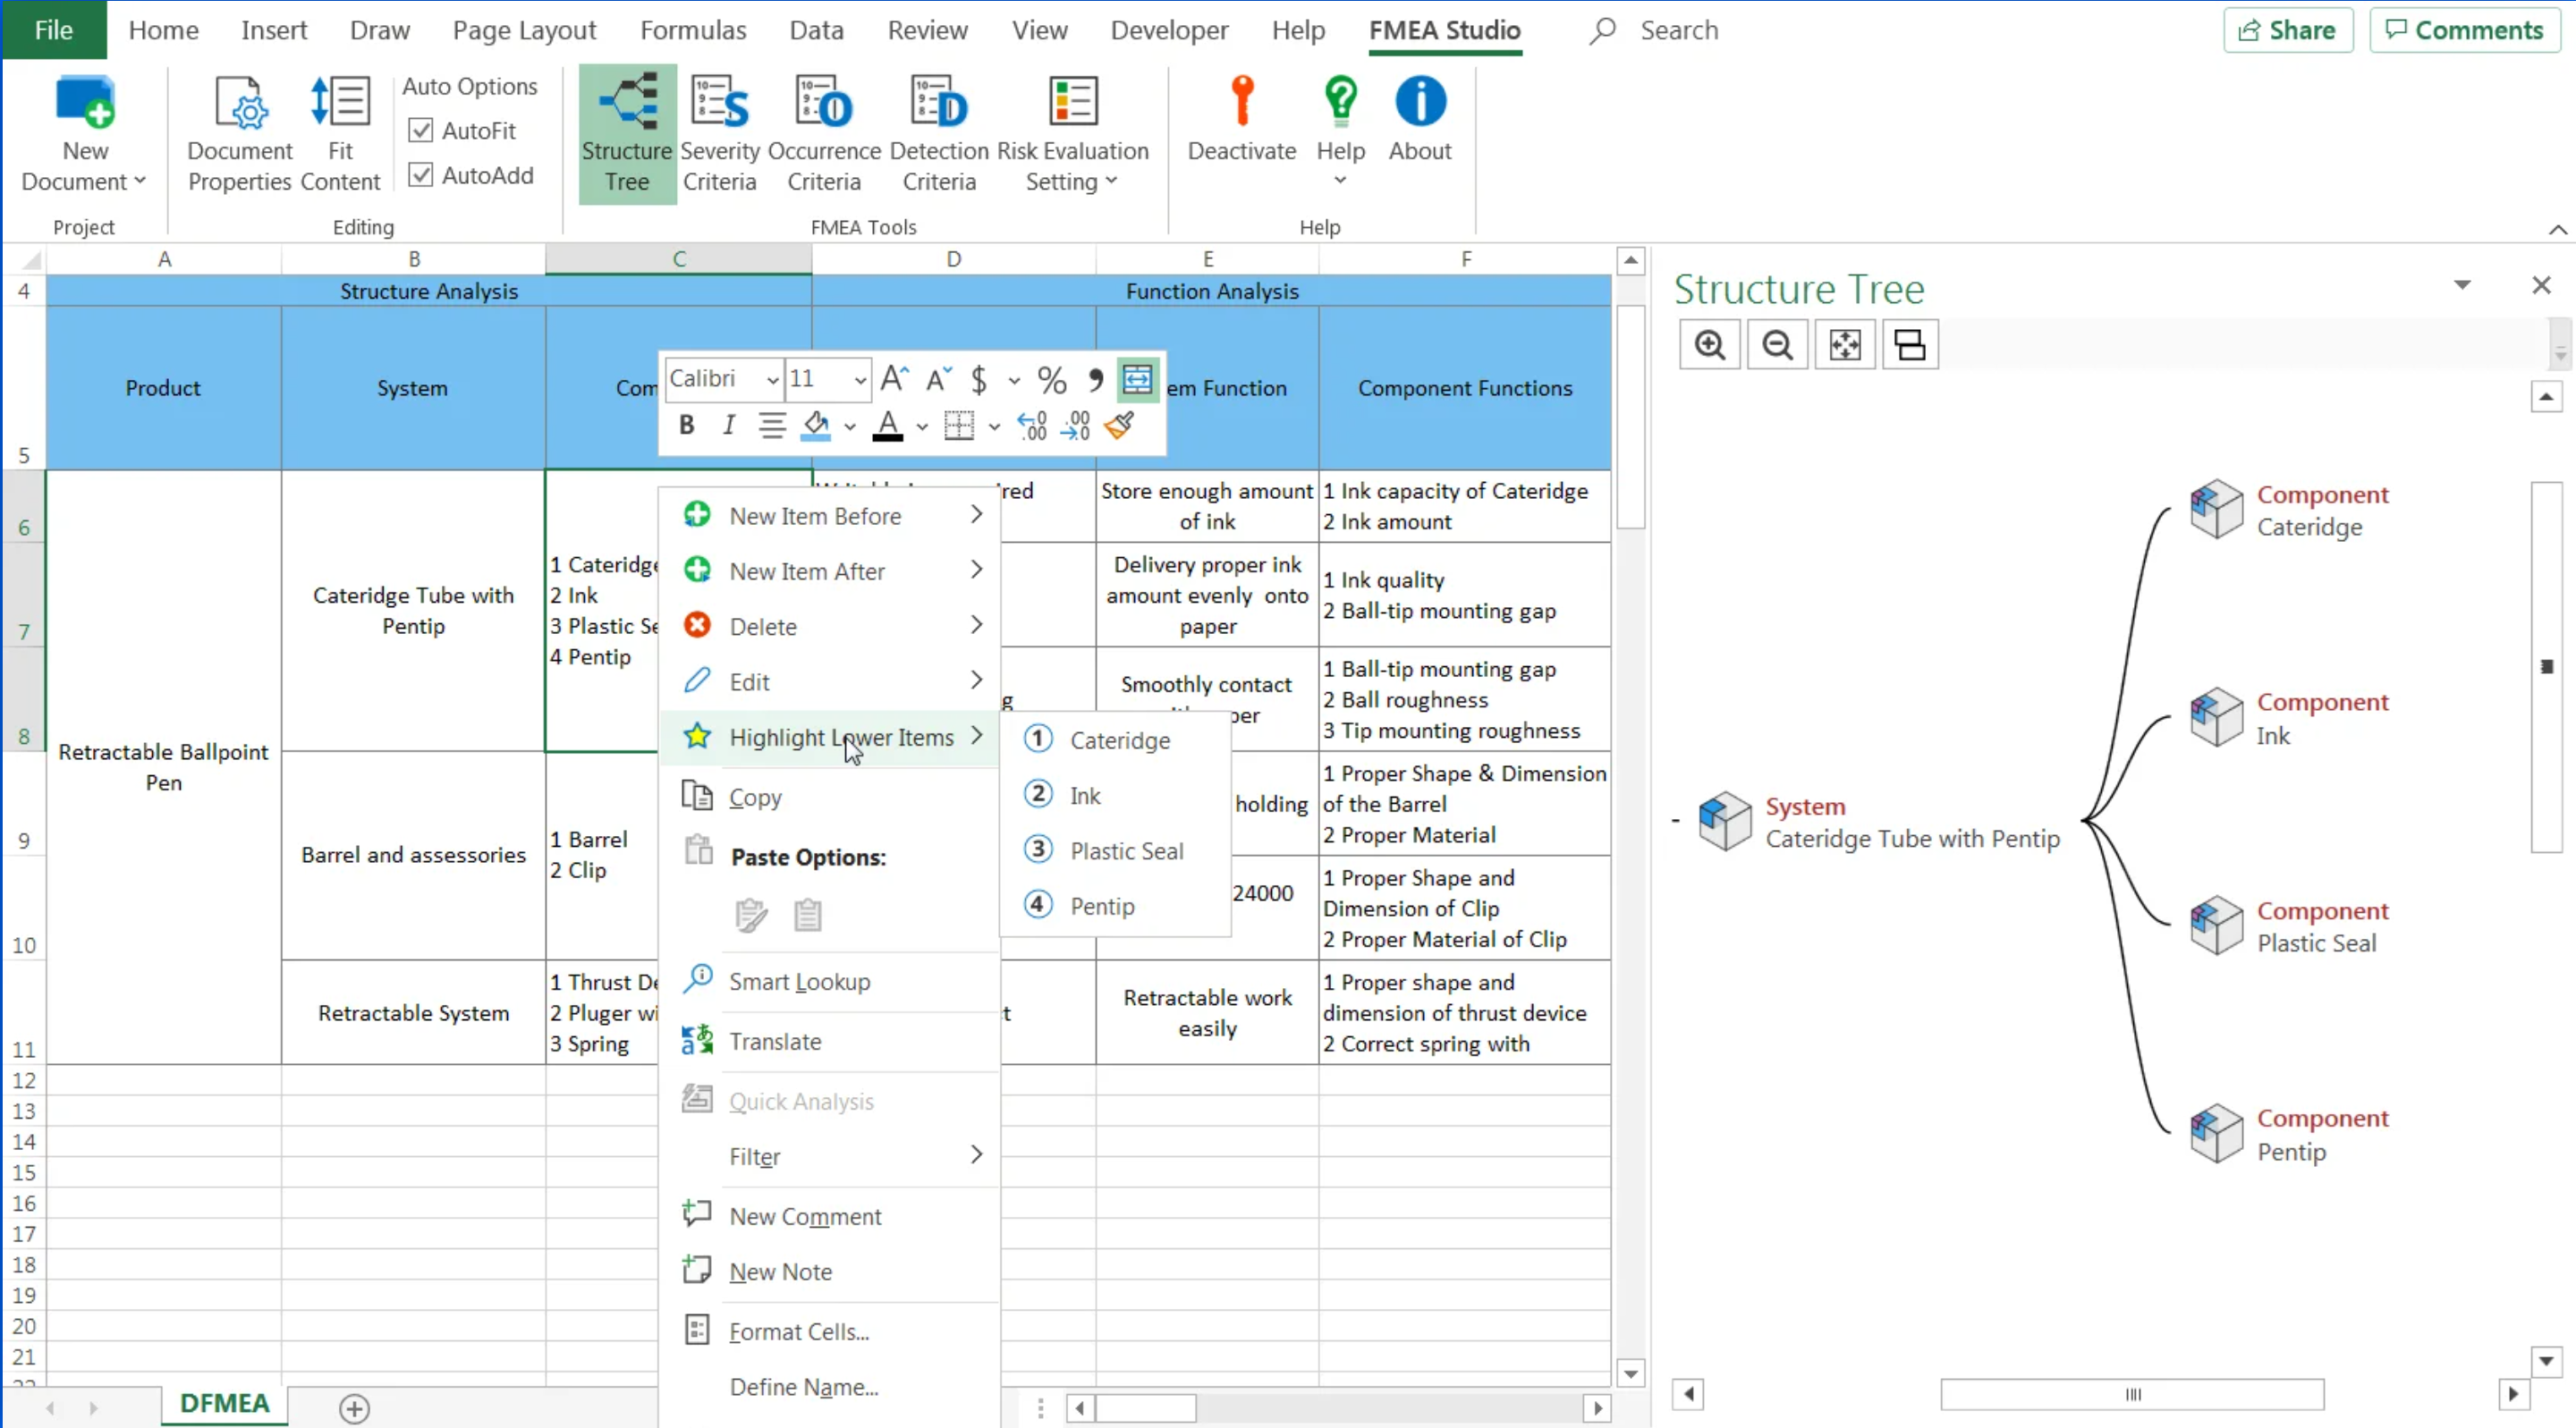
\includegraphics[width=1.0\textwidth]{Figures/iqa.PNG}
	\caption{Nástroj FMEA Sudio }
	\label{fig:iqa}
\end{figure}

\cite{fmeaStudio}FMEA Studio slouží jako nadstavba výše zmíněného způsobu tvorby analýzy pomocí tabulkového editoru. Tento nástroj slouží jako rozšíření například do programu Microsfot Excel, kde pak nabízí například několik různých šablon zaměřených zejména na Návrh a Proces. Samozřejmostí je také automatický výpočet RPN a určení AP. Uživatel má také možnost nastavení vlastních měřítek pro hodnocení atributů Význam, Výskyt a Detekce. Dokonce je možné zobrazit relace mezi daty i pomocí stromové struktury. Další užitečnou funkcí je možnost nastavení priority jednotlivých hodnotících atributů pro jednodušší určení do jakého stavu identifikováné riziko přejde. Nástroj také nabízí základní zobrazení výstupu analýzy pomocí matice rizik a grafů. Formatování je umožněno zejména pomocí hostitelského programu. Ukázku tohoto rozšíření je možné vidět na obrázku \ref{fig:iqa}
\break
\break


\subsection{PQ-FMEA}
\cite{pqFMEA}PQ-FMEA je čistě desktopová aplikace pro tvorbu FMEA. Tato aplikace umožňuje tvorbu dvou základních typů(DFEMA, PFMEA) a podporuje práci s typy RPFMEA, LFMEA, MFFMEA, SwFMEA, UFMEA. Aplikace nabízí docela široké možnosti, co se týká zobrazení dat. Tabulku lze zobrazit dle standardu AIAG nebo VDA nebo jejich společné variantě. Dále lze také zobrazit kontrolní plán, což je dokument, který se z pravidla vypracovává po ukončení práce na analýze zaměřené na proces. Tento nástroj také disponuje zajímavou možností tvorby analýzy v grafickém režimu. V prvé řadě lze přepínat mezi třemi módy, které určují krok analýzy. Po výběru módu lze tvořit relace mezi prvky stylem drag\&drop. U prvního módu reprezentující strukturální analýzu je tento způsob velice účinný. Nicméně u dalších dvou módu reprezentující funkční analýzu a analýzy selhání se zobrazují v rámci sloupců kombinace atributů z předchozích kroků a celý proces je tak velice nepřehledný. Také zobrazení pomocí tabulky není úplně nejpřívětivější. V rámci kroků analýzy nejsou nijak barevně rozlišeny prvky, které spolu souvisí a pro zobrazení relací chybí slučovaní buněk tabulky. Na druhou stranu tato aplikace nabízí velikou škálu vstupních a výstupních funkcí jako je:
\begin{itemize}
    \item Nastavení vlastních měřítek pro určení hodnotících atributů spolu s možností jejich importu a exportu
    \item Tvorba logů ze setkání a přidělování úkolu jednotlivým uživatelům
    \item Zobrazení výstupních grafů analýzy, matice rizik, rozložení rizik podle AP 
    \item Tisk jednotlivých částí analýzy
    \item Možnost vyhledávání v tabulce podle klíčového slova
    \item Podporu několika světových jazyků
\end{itemize}

Jedná se tak o docela robustní nástroj s širokou škálou funkcí nicméně podle názoru autora této práce s několika základními nedostaky. Ukázku této aplikace je možné vidět na obrázku \ref{fig:pq}

\begin{figure}[h]
\centering
	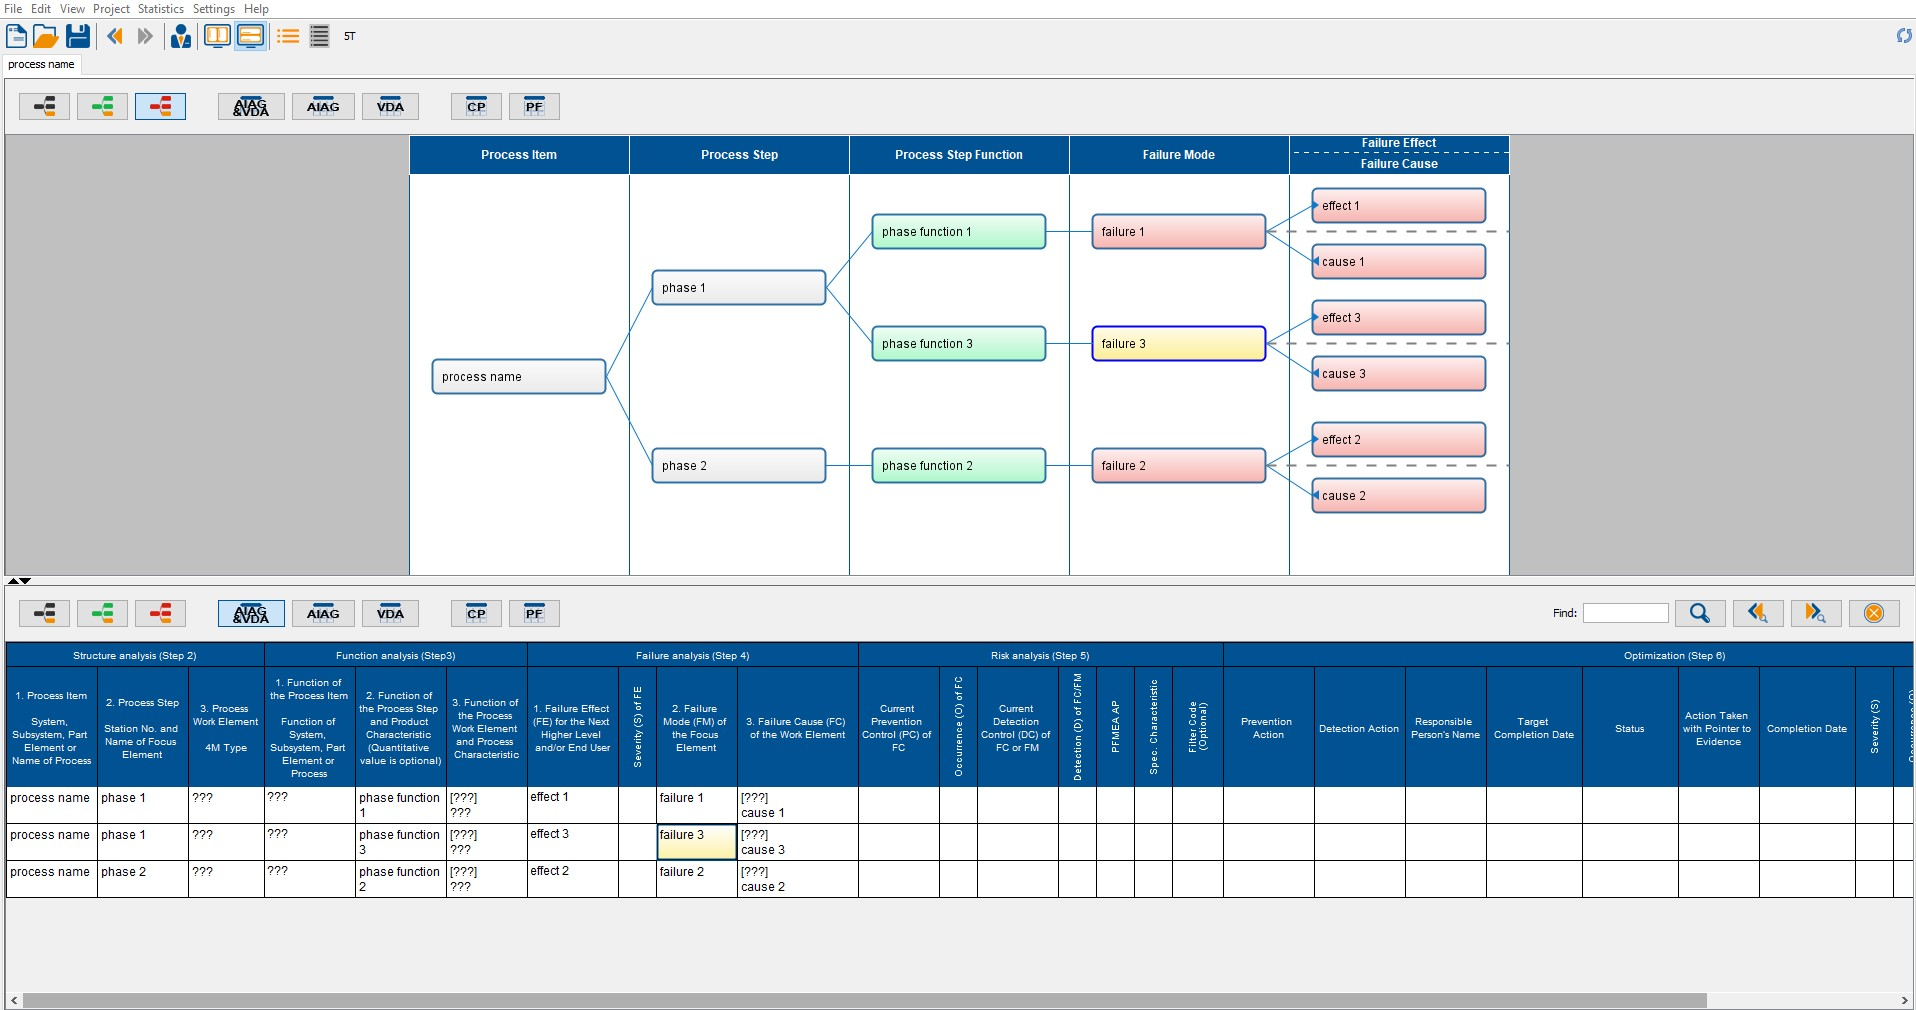
\includegraphics[width=1.0\textwidth]{Figures/pq.jpg}
	\caption{Nástroj PQ-FMEA }
	\label{fig:pq}
\end{figure}

\subsection{Relyence FMEA}
\cite{relyenceFMEA}U předchozích dvou nástrojů se jednalo o desktopová řešení, kterým chyběla přímá podpora pro možnost sdílené práce na analýze více uživatelů. Tento problém by šel případně vyřešit za pomocí externích programů pro sdílení plochy jednoho z uživatelů a také samostatného sdílení souborů analýzy. Správným směrem se vydala společnost Relyence, která vytvořila aplikaci webovou. Tato apliakce nabízí kromě tvorby FMEA analýzy také několik dalších method z oblasti Risk Managementu jako je například Fault Tree, Reliabity Prediction apod. V rámci FMEA aplikace podporuje typy DFMEA, PFMEA, FMEA-MSR, FMECA. Tyto typy ovšem neodpovídají standardu AIAG/VGA pro automobilový průmysl. Aplikace sice nedisponuje grafickým zobrazením dat analýzy, ale nabízí opravdu komplexní možnosti práce s tabulkou. Také je možné grafické zobrazení a tvorba podpůrných souvisejích artefaktů jako je Boundary diagram nebo P-diagram. Samozřejmostí je také import a export dat analýzy do několika podporovaných formátů. Tento nástroj, narozdíl od dvou předchozích, určitým způsobem řeší správu uživatelů. Je zde možné si vytvořit uživatelský účet a ukládat si data analýzy. Zajímavostí je, že webová aplikace by měla být podle všeho také podporovat zobrazení na zařízení jako je tablet nebo dokonce mobilní zařízení. Ani u této apliakce ovšem nevypadá, že by existovali nějaké sofistikovanější možnosti společné práce na analýze. Ukázku této aplikace možné vidět na obrázku  \ref{fig:relyence}

\begin{figure}[h]
\centering
	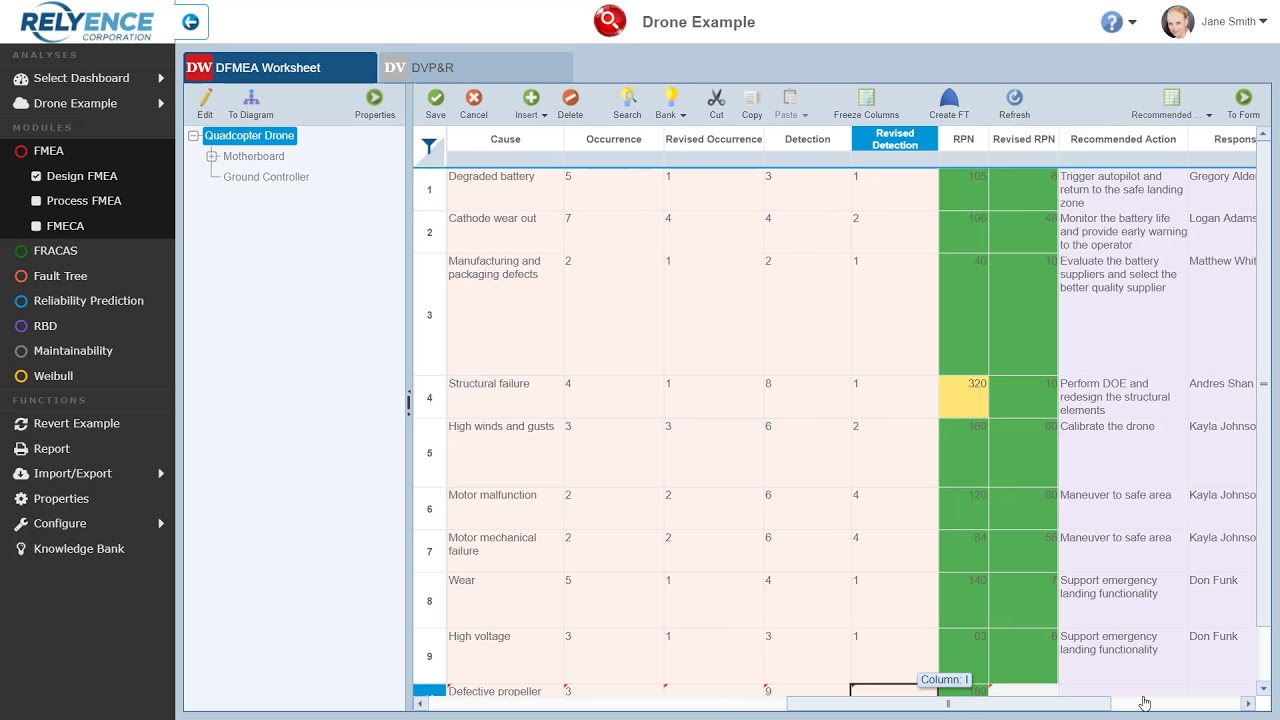
\includegraphics[width=1.0\textwidth]{Figures/relyence.jpg}
	\caption{Nástroj Relyence FMEA }
	\label{fig:relyence}
\end{figure}

\section{Srovnání dostupných řešení}
V této části kapitoly budou srovnány výše uvedené nástroje pro tvorbu FMEA, které jsou dostupné na trhu. Součástí tohoto srovnání bude i nástroj, který byl vytvořen v rámci této diplomové práce. Důvodem je ukazát, jak byly jednotlivé požadavky na nástroj realizovány v porovnání s ostatními komerčními produkty. Dále následuje tabulka \ref{tab:compare}, kde lze vidět na základě jakých požadavků byly nástroje posouzeny a jak je jednotlivé řešení naplňují.
\break
\break
\break
\break
\break
\break

\begin{longtable}{|p{4cm} | p{12cm} |} 
        \caption{Srovnání dostupných řešení}
\label{tab:compare}
         \hline
& \textbf{1. Tvorba analýzy podporující typy DFMEA, PFMEA,...} \\ \hline
 FMEA Studio &	DFMEA,PFMEA, Software FMEA  \\ 
 PQ-FMEA &	 DFMEA,PFMEA  \\ 
 Relyence FMEA &	 DFMEA,PFMEA, FMECA, FMEA-MSR  \\ 
Vlastní řešení &	 DFMEA,PFMEA \\ \hline

& \textbf{2. Zobrazení dat analýzy pomocí textové tabulky.}  \\ \hline
 FMEA Studio &	Rozšíření tabulkového editoru + přidané některé vlastní funkce, správné slučování buněk, nedostatečné barevné rozlišení souvisejících atributů.  \\ 
 PQ-FMEA &	 Různé možností zobrazení, špatné slučování buněk, nedostatečné barevné rozlišení souvisejích atributů.  \\ 
 Relyence FMEA &	 Pokročilé funkce práce s tabulkou, správné slučování buněk na základně relací mezi atributy.  \\ 
Vlastní řešení &	 Zobrazení a následně i editace dat tabulky, zobrazení relací slučováním buněk, rozšířené barevné rozlišení souvosejích atributů s možností označení jednotlivých prvků ze strukturální analýzy. \\ \hline

& \textbf{3. Zobrazení dat analýzy v grafickém režimu.} \\ \hline
 FMEA Studio &	 Možnost zobrazit strukturu dat v jednotlivých krocích na samostatném panelu, přidávání i editace prvků.\\ 
 PQ-FMEA & Náhled i tvorba pomocí tří módu zobrazení stromovou strukturou, lehce nepřehledné v rámci některých módů, tvorba stylem drag\&drop a úpravá prvků.  \\ 
 Relyence FMEA &	 NE  \\ 
Vlastní řešení &	 Možnost tvorby stromové struktury, následně přidávání funkcí a selhání jednotlivým prvků ze struktury pomocí modálních oken, zoom, skrytí/zobrazení potomků. \\ \hline

& \textbf{4. Soubežná práce více uživatelů.} \\ \hline
 FMEA Studio &	Za pomocí externího software + sdílení souboru analýzy.  \\ 
 PQ-FMEA &	 Za pomocí externího software + sdílení souboru analýzy. \\ 
 Relyence FMEA &	  Základní práce s uživatelskými účty, jinak pomocí externího SW + sdílení souborů.  \\ 
Vlastní řešení &	 Možnost připojení několika uživatelů do skupin na základě stejného odkazu a sdílení prováděných změn v reálném čase. Registrace a přihlašování uživatelů. \\ \hline
& \textbf{5. Možnost export a importu dat analýzy. } \\ \hline
 FMEA Studio &	Pouze ukládání a načítaní souboru tabulkového editoru.  \\ 
 PQ-FMEA &	  Ukládání a načítání dat analýzy do vlastního formátu, import a export nastavení vlastních měřítek pro hodnocení.   \\ 
 Relyence FMEA &	 Ukládání a načítání dat analýzy do vlastního formátu.  \\ 
Vlastní řešení &	 Ukládání a načítaní dat analýzy do JSON formátu, export do formátu .xls, .png.\\ \hline

& \textbf{6. Další podpůrné funkce(nastavení vlastních měřítek hodnocení, grafy na výstupu)} \\ \hline
 FMEA Studio &	Nastavení vlastních měřítek pro hodcnocení, hranic pro hodnocení rizik, výstupní grafy a matice rizik, flow diagram,...  \\ 
 PQ-FMEA &	 Nastavení vlastních měřítek pro hodcnocení, výstupní grafy a matice rizik, tisk formulářů, logování a přidělování úkolů uživatelům.  \\ 
 Relyence FMEA &	  Možnost importu a tvorby několika souvisejících diagramů. \\ 
Vlastní řešení &	  Nastavení vlastních měřítek pro hodnocení, tvorba logů ze setkání, kontrola dokončení všech nalezených rizik. \\ \hline
\end{longtable}

Závěrem tohoto popisu lze říci, že ač nalezené nástroje obsahují několik dostupných typů FMEA, různých možností nastavení projektů, výstupních grafů a matic, tak postrádají jednu ze základních funkcí a to umožnit týmu provádějící analýzu souběžnou a efektivní práci na analýze přímo skrze používáný nástroj. To je nesporná výhoda nástroje, který byl vytvořen v rámci této práce. Další výhodou je, že vytvořený nástroj celkem jasně sdružuje atributy, které spolu souvisí, kdy u jiných nástrojů nejsou jednotlivé souvislosti hned na první pohled jasné. Následuje kapitola \ref{sec:navrh}, která již bude zaměřena vyvýjený nástroj, nejdříve jeho návrh a architekturu. 
 